\documentclass{lug}
\usepackage{graphicx}
\usepackage{amsmath}
\usepackage{bm}
\usepackage{color}
\def\code#1{\texttt{#1}}

\title{Pattern Discovery in Brain Imaging Genetics via SCCA Modeling with a  Generic Non-convex Penalty}
\author{Lei Du, Kefei Liu, Xiaohui Yao, Jingwen Yan, Shannon L. Risacher, Junwei Han, Lei Guo, Andrew J. Saykin, Li Shen and the ADNI}
\institute{\textbf{Presented By:} \\ Lou Brand \\ Department of Computer Science\\Colorado School of Mines}
\date{\today}

\begin{document}

\section{Background/Motivation}
\frame{
    \frametitle{Biology Perspective}
    \center{
        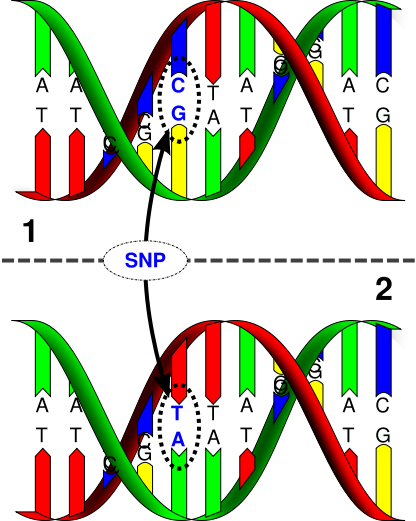
\includegraphics[scale=0.3]{images/snp.png}
        \hspace{.5cm}
        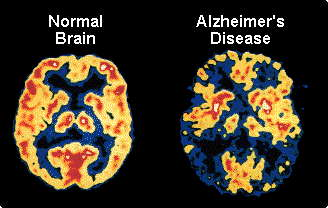
\includegraphics[scale=0.6]{images/brain.jpg}
    }
}

\frame{
    \frametitle{Machine Learning Perspective - Regularization}
    \center{
        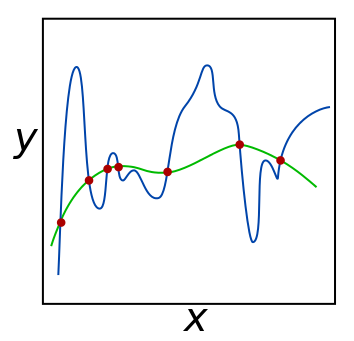
\includegraphics[scale=.5]{images/regularization.png}\\
        $\min\limits_f \sum\limits_{i=1}^{n} V(f(x_i), y_i) + \lambda R(f) $
    }
}

\frame{
    \frametitle{$\ell_1$-norm vs. $\ell_2$-norm}
    Consider the vector: $ \mathbf x=(1,\varepsilon)\in\mathbb{R}^2 $ where $ \varepsilon>0 $ is small.\\ 
    \pause
    $\ell_1$-norm: $$||\mathbf x||_1 = 1+\varepsilon$$
    $\ell_2$-norm: $$||\mathbf x||_2^2 = 1+\varepsilon^2$$
    \pause
    Suppose we reduce the magnitude of $x_1$ to $1 - \delta$, where $\delta\leq\varepsilon$:
    $$||\mathbf x-(\delta,0)||_1 = 1-\delta+\varepsilon,\ \ ||\mathbf x-(\delta,0)||_2^2 = 1-2\delta+\delta^2+\varepsilon^2$$
    \pause
    Instead, suppose we reduce the magnitude of $x_2$ to $\varepsilon - \delta$:
    $$ ||\mathbf x-(0,\delta)||_1 = 1-\delta+\varepsilon,\ \ ||\mathbf x-(0,\delta)||_2^2 = 1-2\varepsilon\delta+\delta^2+\varepsilon^2$$
}

\frame{
    \frametitle{$\ell_1$-norm vs. $\ell_2$-norm}
    \center{
        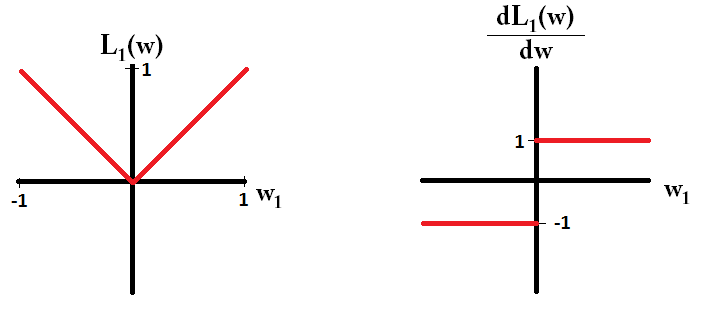
\includegraphics[scale=0.35]{images/l1graph.png}\\
        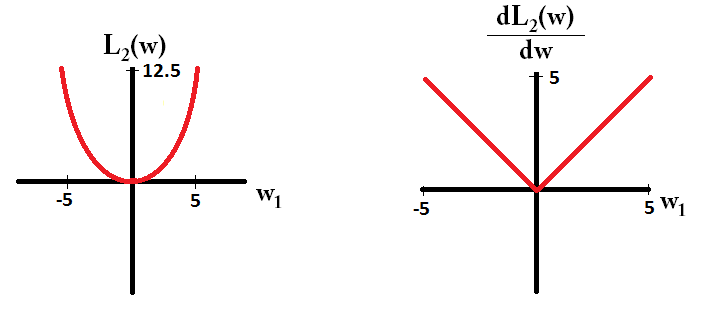
\includegraphics[scale=0.35]{images/l2graph.png}\\
        $\ell_1$-norm has some nice properties (sparsity, convex, etc.) but can we find a better regularization term? One that doesn't penalize large coefficients?
    }
}



\section{Approach}
\frame{
    \frametitle{Properties of a ``Good" Penalty Function}
    \begin{itemize}[<+->]
        \item Singular at the origin; this will encourage sparsity. 
        \item Continuous models == Stable model selection
        \item Should not penalize large coefficients
    \end{itemize}
    \pause
    \center{
        \textbf{Side Note:} Solving $\ell_0$-norm constrained problems is NP-hard
    }
}

\frame{
    \frametitle{Sparse Canonical Correlation Analysis (SCCA)}
    Let $\mathbf X\in \mathcal{R}^{n\times p}$ be a matrix representing the SNP biomarkers data. Let $\mathbf Y\in \mathcal{R}^{n\times r}$ be a matrix representing the brain imaging data. 
    \pause
    The SCCA model is defined as:
    $$ \min_{\mathbf u,\mathbf v}-\mathbf u^{\mathrm T} \mathbf X^{\mathrm T}\mathbf Y\mathbf v$$
    $$s.t.  {\Arrowvert\mathbf X\mathbf u\Arrowvert}^2\leq1,{\Arrowvert\mathbf Y\mathbf v\Arrowvert}^2\leq1,\mathrm\Omega(\mathbf u)\leq c_1,\mathrm\Omega(\mathbf v)\leq c_2$$
    In this case the $\mathrm\Omega(\mathbf u)$ and $\mathrm\Omega(\mathbf v)$ are arbitrary convex regularization functions tuned via $c_1$ and $c_2$. 
    \pause
    \center{
        \textbf{Opportunity:} Apply non-convex regularization to SCCA:
    }
    $${\mathrm\Omega}_\mathrm{nc}(\mathbf u)=\sum_{i=1}^pP_{\lambda,\gamma}(\vert u_i\vert)$$
}

\frame{
    \frametitle{Non-convex SCCA: Penalty Functions}
    \center{
        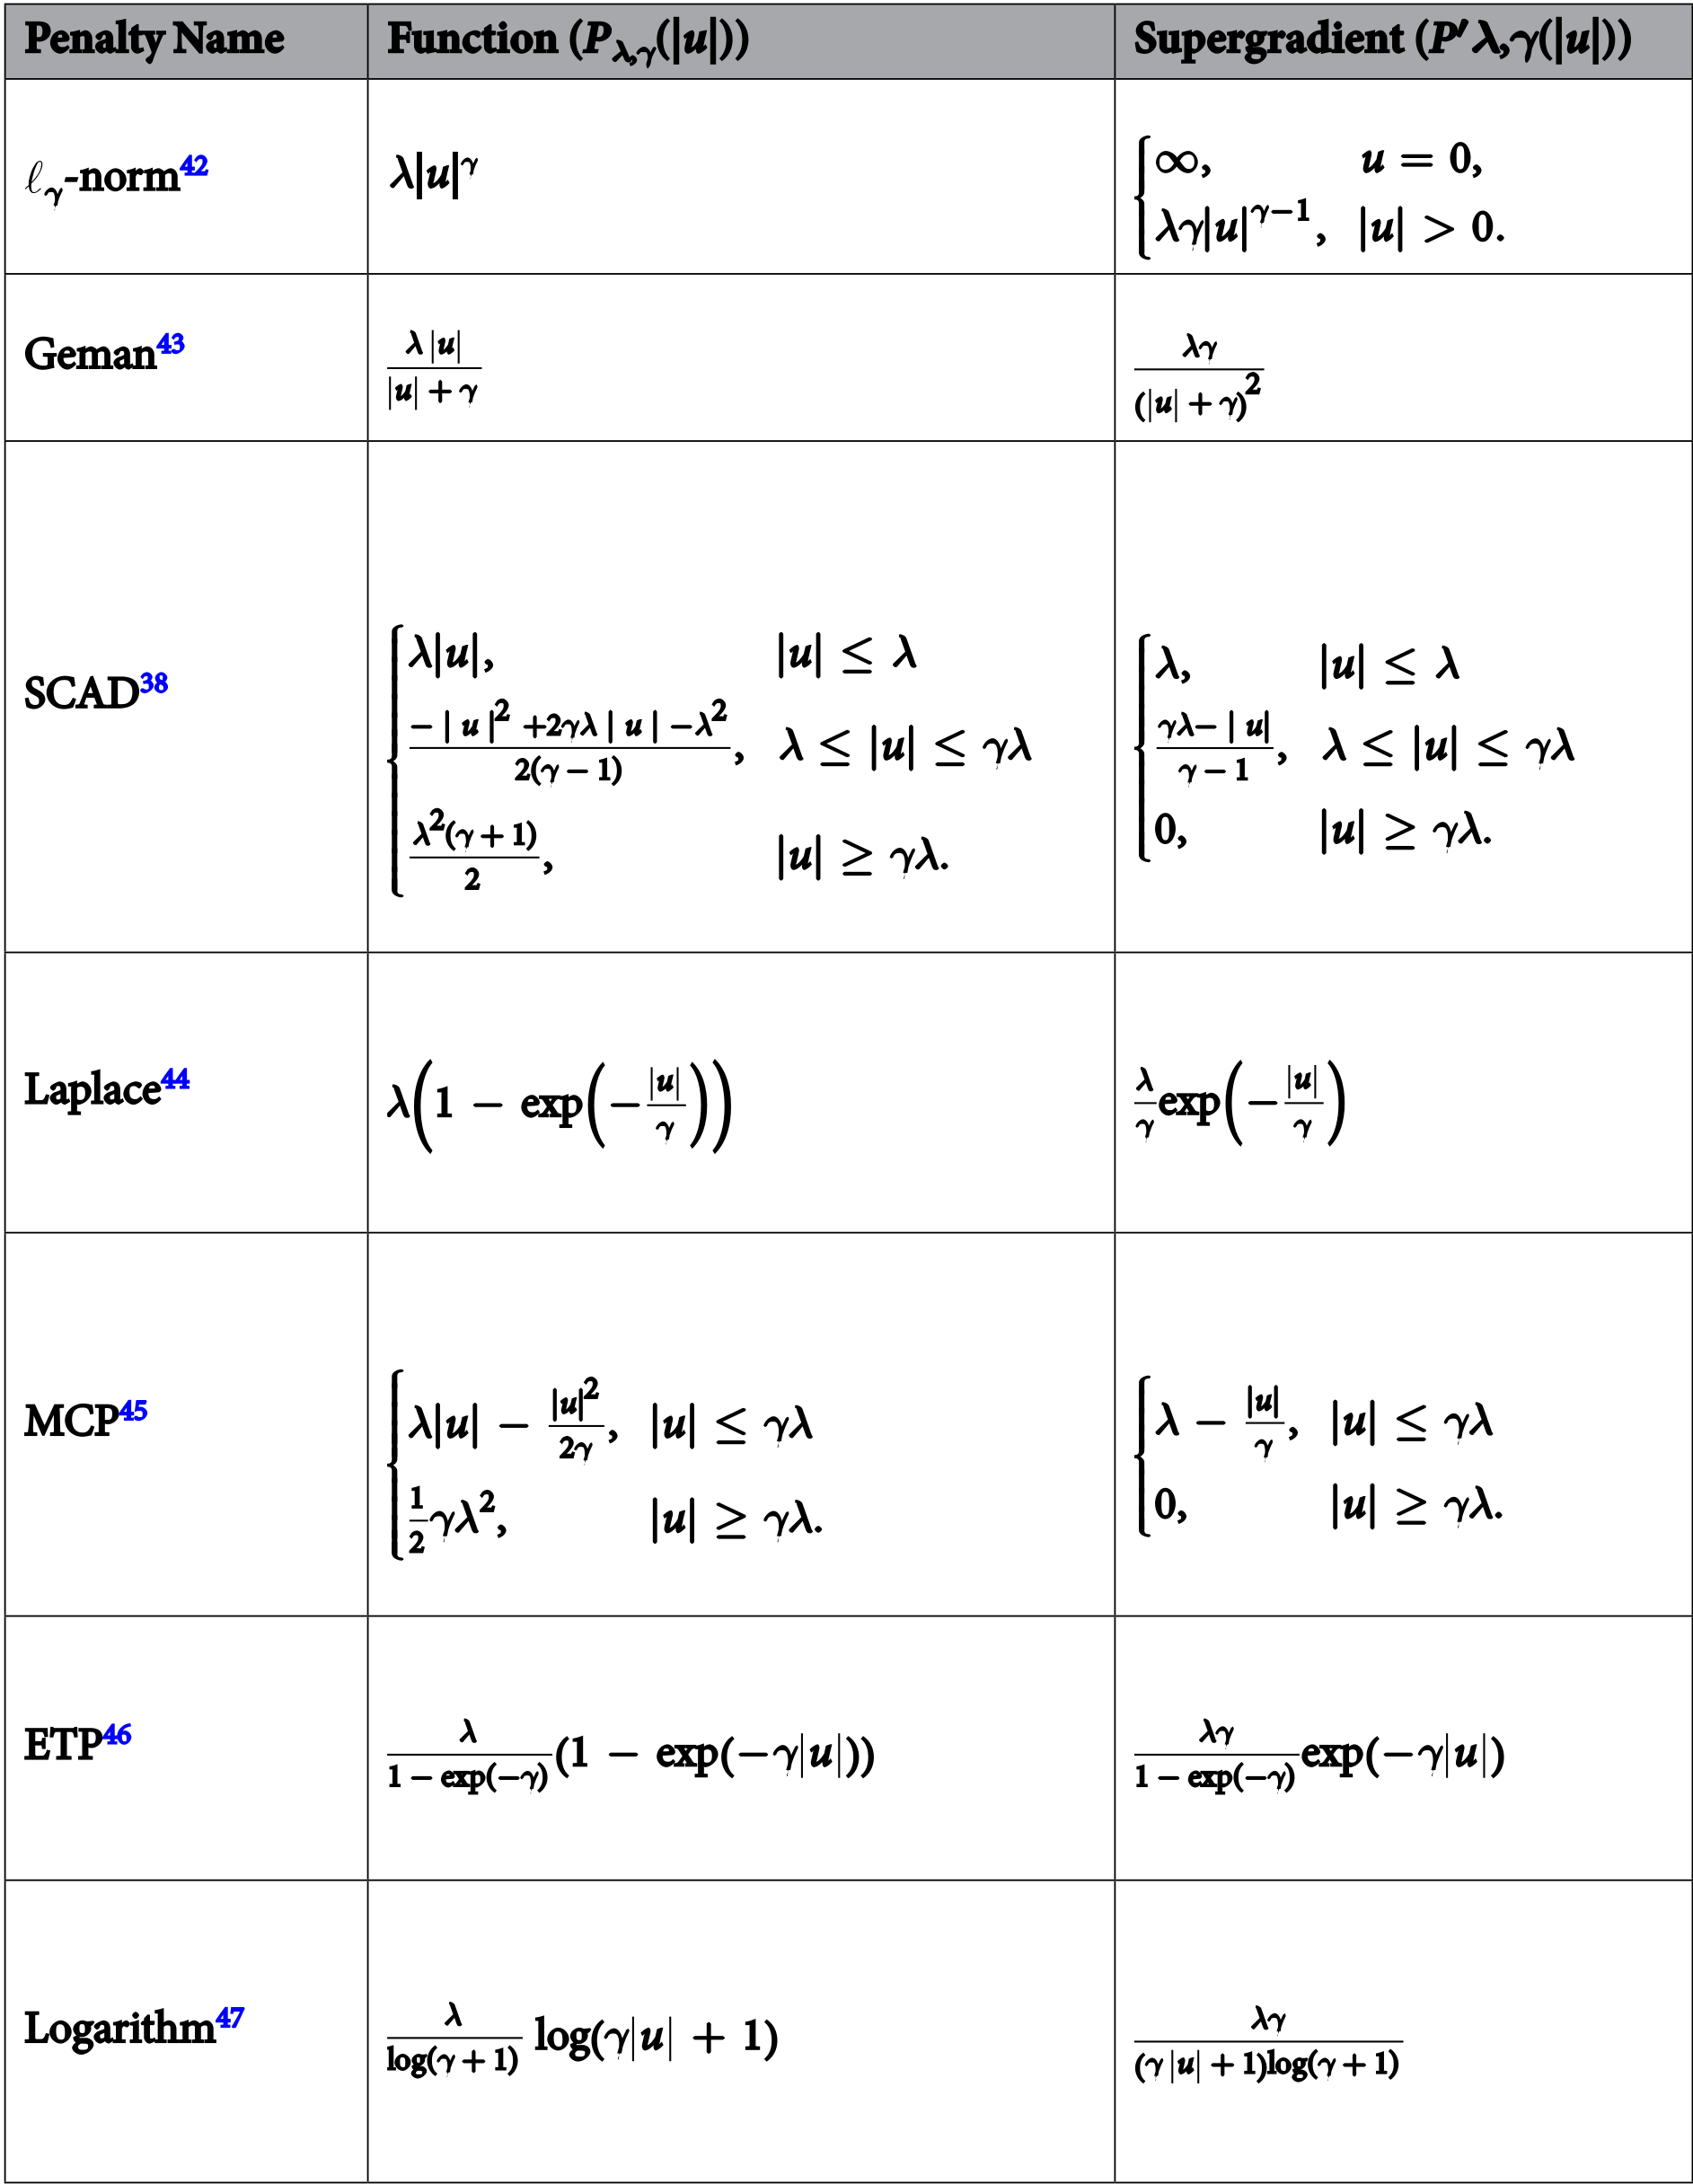
\includegraphics[scale=0.6]{images/table1.png}
    }
}

\frame{
    \frametitle{Non-convex SCCA: Penalty Functions}
    \center{
        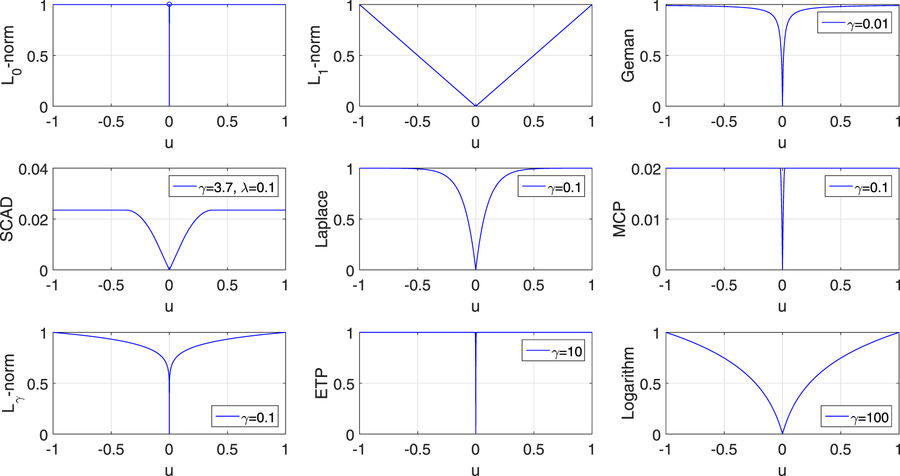
\includegraphics[scale=1.4]{images/fig1.jpg}
    }
}

\frame{
    \frametitle{Non-convex SCCA}
    The non-convex SCCA model is defined as:
    $$\min_{\mathbf u,\mathbf v}-\mathbf u^{\mathrm T}\mathbf X^{\mathrm T}\mathbf Y\mathbf v+{\mathrm\Omega}_\mathrm{nc}(\mathbf u)+{\mathrm\Omega}_\mathrm{nc}(\mathbf v)$$
    $$s.t.  {\Arrowvert\mathbf X\mathbf u\Arrowvert}^2\leq1,{\Arrowvert\mathbf Y\mathbf v\Arrowvert}^2\leq1$$
    \pause
    To solve we apply the Lagrangian method (and remove constants): 
    $$\mathcal{L}\boldsymbol(\mathbf u\boldsymbol,\mathbf v\boldsymbol)=-\hspace{-.25em}\mathbf u^\mathrm T\mathbf X^\mathrm T\mathbf Y\mathbf v+{\mathrm\Omega}_\mathrm{nc}(\mathbf u)+{\mathrm\Omega}_\mathrm{nc}(\mathbf v)+\frac{\alpha_1}2{{\Arrowvert\mathbf X\mathbf u\Arrowvert}^2}+\frac{\alpha_2}2{{\Arrowvert\mathbf Y\mathbf v\Arrowvert}^2}$$
    \pause
    \center{
        Next, we would like to transform $\mathrm\Omega_\mathrm{nc}$ into a convex function... 
    }
}

\frame{
    \frametitle{Non-convex SCCA: Local Quadratic Approximation (LQA)}
    Given the first-order Taylor expansion of $P_{\lambda_1,\gamma}(\sqrt\mu)$ at $\mu_0$, where $\mu$ and $\mu_0$ are estimates at two successive iterations:
    $$P_{\lambda,\gamma}(\sqrt\mu)\approx P_{\lambda,\gamma}(\sqrt{\mu_0})+P'_{\lambda,\gamma}(\sqrt{\mu_0})\frac1{2\sqrt{\mu_0}}(\mu-\mu_0)$$
    \pause
    Substitute $\mu = u_i^2$ and $\mu_0 = (u_i^t)^2$:
    $$P_{\lambda,\gamma}(\vert u_i\vert)\approx P_{\lambda,\gamma}(\vert u_i^t\vert)+P'_{\lambda,\gamma}(\vert u_i^t\vert)\frac1{2|u_i^t\vert}(u_i^2-{(u_i^t)}^2)$$
    \pause
    It follows that:
    $${\mathrm\Omega}_\mathrm{nc}(\mathbf u)=\sum_{i=1}^pP_{\lambda,\gamma}(\vert u_i\vert)\approx\sum_{i=1}^p\frac{P'_{\lambda,\gamma}(\vert u_i^t\vert)}{2|u_i^t\vert}u_i^2+C_\mathbf u$$where,
    $$C_\mathbf u=\sum_{i=1}^p=\left[P_{\lambda,\gamma}(\vert u_i^t\vert)-\frac12P'_{\lambda,\gamma}(\vert u_i^t\vert)\vert u_i^t\vert\right]$$
}

\frame{
    \frametitle{Non-convex SCCA: Local Quadratic Approximation (LQA)}
    The same steps can be applied to ${\mathrm\Omega}_\mathrm{nc}(\mathbf v)$:
    $${\mathrm\Omega}_\mathrm{nc}(\mathbf v)=\sum_{j=1}^qP_{\lambda,\gamma}(\vert v_j\vert)\approx\sum_{j=1}^q\frac{P'_{\lambda,\gamma}(\vert v_j^t\vert)}{2|v_j^t\hspace{-0.25em}|}v_j^2+C_\mathbf v$$
    \pause
    Substitution into $\mathcal{L}\boldsymbol(\mathbf u\boldsymbol,\mathbf v\boldsymbol)$:
    $$\begin{array}{lcc}\arg\hspace{.25em}\min\mathcal{L}\boldsymbol(\mathbf u\boldsymbol,\mathbf v\boldsymbol)&=&\arg\hspace{.25em}\min\hspace{.25em}-\mathbf u^{\mathrm T}\mathbf X^{\mathrm T}\mathbf Y\mathbf v+\sum_{i=1}^p\frac{P'_{\lambda_1,\gamma}(\vert u_i^t\vert)}{2|u_i^t\vert}u_i^2\\&&+\hspace{.25em}\sum_{j=1}^q\frac{P'_{\lambda_1,\gamma}(\vert v_j^t\vert)}{2|v_j^t\vert}v_j^2+\frac{\alpha_1}2\vert\vert\mathbf X\mathbf u{\vert\vert}^2+\frac{\alpha_2}2\vert\vert\mathbf Y\mathbf v{\vert\vert}^2\end{array}$$
    \pause
    Using the alternate convex search algorithm:
    $$\begin{array}{lcc}\mathbf u^{t+1}&=&\arg\min_{\mathbf u}-\mathbf u^{\mathrm T}\mathbf X^{\mathrm T} \mathbf Y\mathbf v^t+\sum_{i=1}^p\frac{P'_{\lambda_1,\gamma}(\vert u_i^t\vert)}{2|u_i^t\vert}u_i^2+\frac{\alpha_1}2\vert\vert\mathbf X\mathbf u{\vert\vert}^2,\\\mathbf v^{t+1}&=&\arg\hspace{.25em}\min_{\mathbf v}-{(\mathbf u^{t+1})}^{\mathrm T}\mathbf X^{\mathrm T}\mathbf Y\mathbf v+\sum_{j=1}^q\frac{P'_{\lambda_2,\gamma}(\vert v_j^t\vert)}{2|v_j^t\vert}v_j^2+\frac{\alpha_2}2\vert\vert\mathbf Y\mathbf v{\vert\vert}^2\end{array}$$
}

\frame{
    \frametitle{Non-convex SCCS}
    We can also take the partial derivative of $\mathcal{L}\boldsymbol(\mathbf u\boldsymbol,\mathbf v\boldsymbol)$ w.r.t. $\mathbf u$ and $\mathbf v$: 
    $$\mathbf0\in-\hspace{-.25em}\mathbf X^{\mathrm T}\mathbf Y\mathbf v+(\mathbf D_1^t+\alpha_1\mathbf X^{\mathrm T}\mathbf X)\mathbf u$$
    $$\mathbf0\in-\hspace{-.25em}\mathbf Y^{\mathrm T}\mathbf X\mathbf u+(\mathbf D_2^t+\alpha_2\mathbf Y^{\mathrm T}\mathbf Y)\mathbf v$$
    Where $\mathbf D_1^t$ is (note $\zeta$ is a very small number):
    $$ \mathbf D_1^t(i,i)=\frac{P'_{\lambda_1,\gamma}(\vert u_i \vert)}{\vert u_i\vert+\zeta} $$
    \pause
    It follows:
    $$\mathbf u^{t+1}=(\mathbf D_1^t+\alpha_1\mathbf X^{\mathrm T}\mathbf X)^{-1}\mathbf X^{\mathrm T}\mathbf Y\mathbf v^t$$ 
    $$\mathbf v^{t+1}=(\mathbf D_2^t+\alpha_2\mathbf Y^{\mathrm T}\mathbf Y)^{-1}\mathbf Y^{\mathrm T}\mathbf X\mathbf u^{t+1}$$
}

\frame{
    \frametitle{Algorithm}
    \center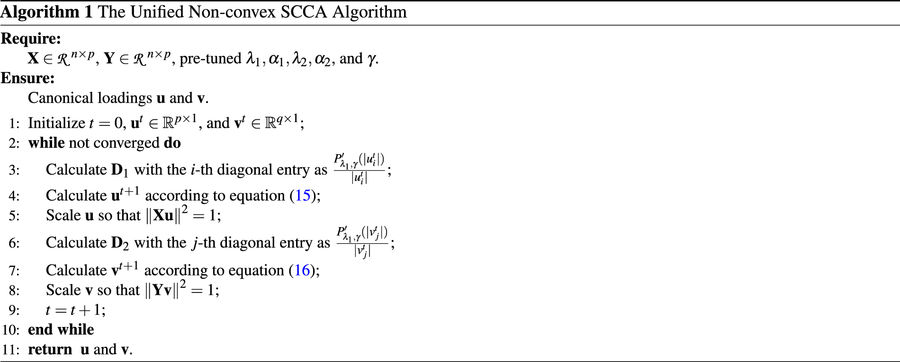
\includegraphics[scale=1.8]{images/algorithm1.jpg}
}


\section{Experiments}
\frame{
    \frametitle{Synthetic Data}
    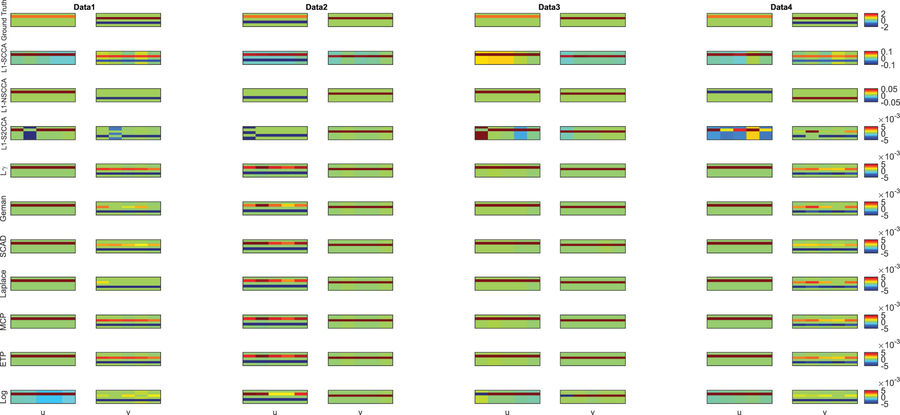
\includegraphics[scale=1.5]{images/fig2.jpg}
}

\frame{
    \frametitle{Synthetic Data (Correlation Coefficients)}
    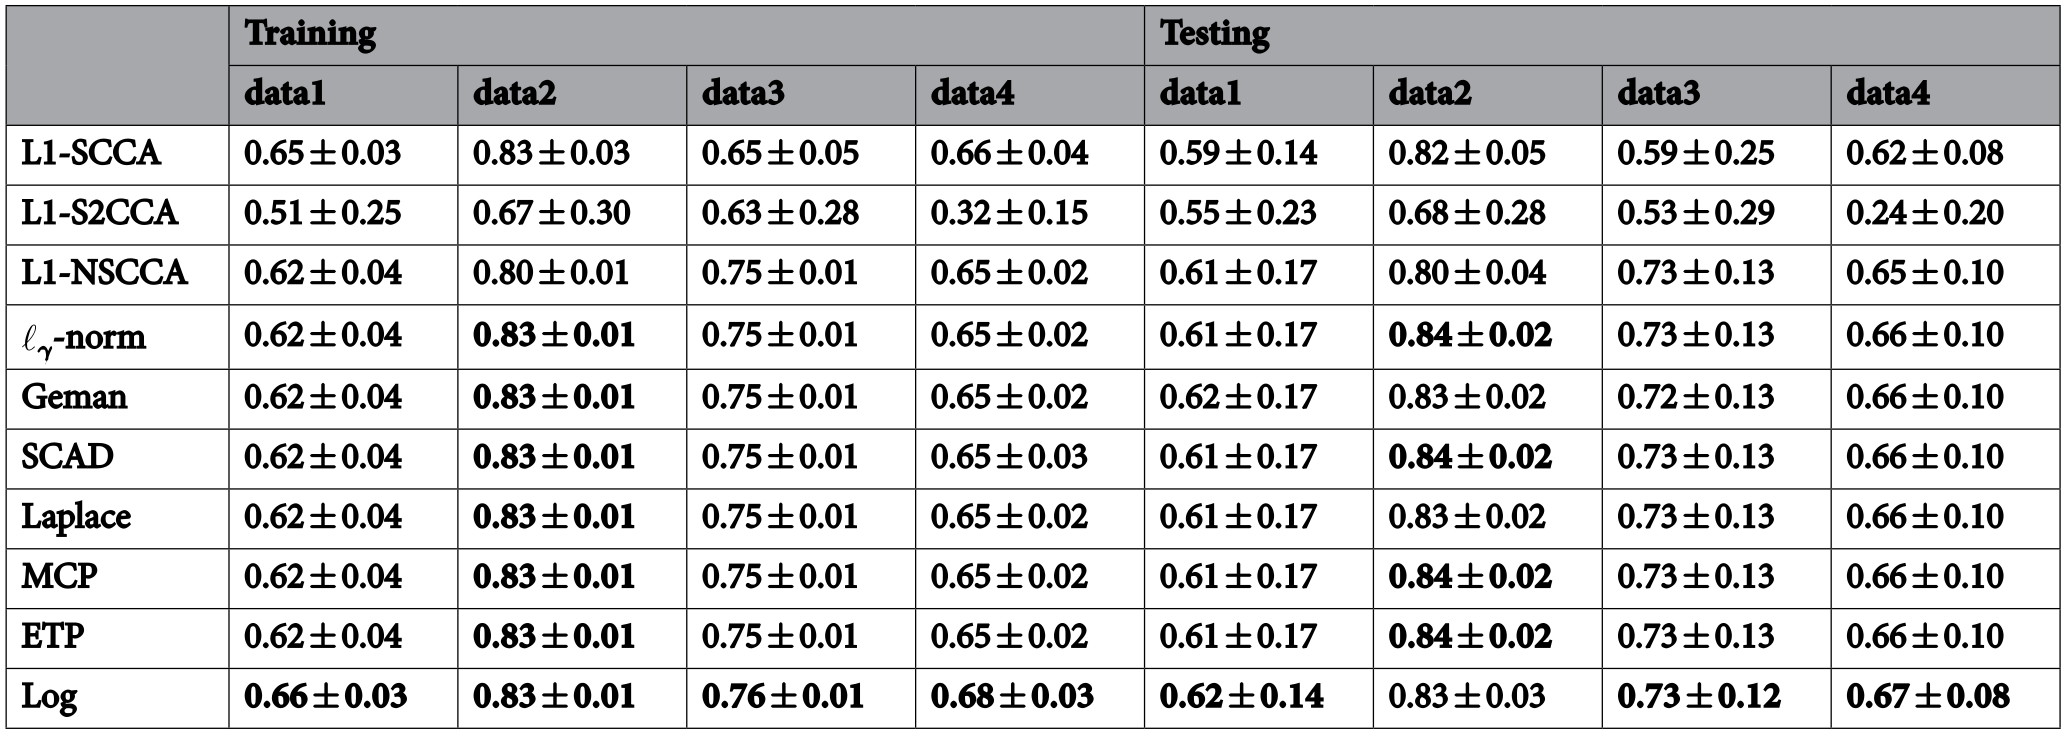
\includegraphics[scale=0.8]{images/table5.png}
}

\frame{
    \frametitle{ADNI Data ($\mathbf u$ and $\mathbf v$)}
    \center{
        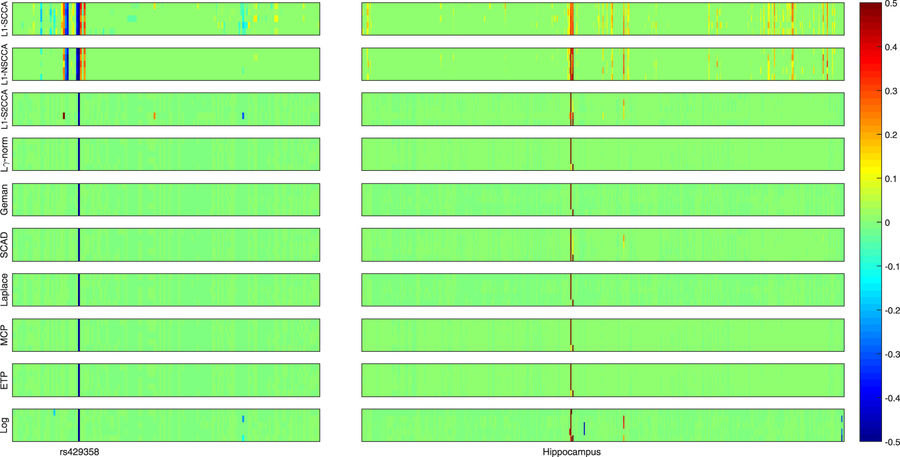
\includegraphics[scale=1.5]{images/fig3.jpg}\\
        \textbf{Key:} The proposed methods increased the sparsity of the solutions
    }
}

\frame{
    \frametitle{ADNI Data ($\mathbf v$ mapped on Hippocampus)}
    \center{
        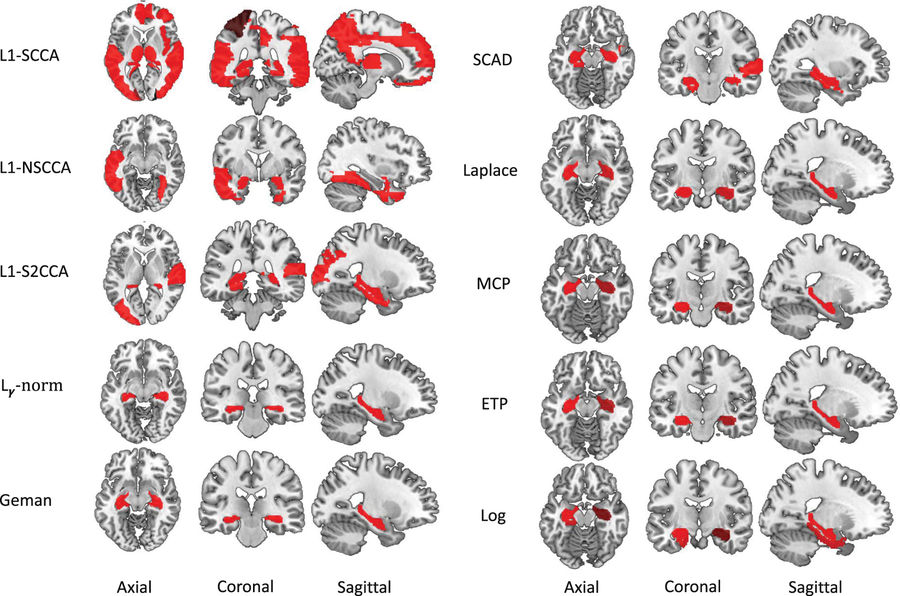
\includegraphics[scale=1.3]{images/fig4.jpg}\\
        \textbf{Takeaway:} The proposed methods generate a cleaner signal than $\ell_1$-norm based methods
    }
}

\section{Conclusions}
\frame{
    \frametitle{Desirable Properties}
    \begin{itemize}[<+->]
        \item Concave
        \item Piecewise continuous
        \item Piecewise differentiable
        \item Effective + fast (due to $\ell_2$ approximation using LQA)
        \item Doesn't over penalize large coefficients
        \item Generates sparse solutions
        \item \textbf{Con:} Tuning parameters ($\lambda_1$, $\alpha_1$, $\lambda_2$, $\alpha_2$, $\gamma$)
    \end{itemize}
}

\frame{
    \begin{center}
        \Huge{Questions/Discussion}
    \end{center}
}

\nocite{*} % Include everything in the .bib file.
\bibliographystyle{plainnat}
\bibliography{non-convex-scca}

% that's all, folks
\end{document}
